\documentclass{article}
\usepackage{cmap}
\usepackage[T2A]{fontenc}
\usepackage[utf8]{inputenc}
\usepackage[english,russian]{babel}
\usepackage{setspace}
\usepackage{geometry}
\usepackage{graphicx}
\usepackage{amsfonts}
\graphicspath{{graphicslab1/}}
\DeclareGraphicsExtensions{.pdf, .png, .jpg, .fig}
\geometry{top=2cm}
\geometry{bottom=2cm}
\geometry{left=2cm} % отступ справа
\geometry{right=2cm} % отступ слева

\begin{document}
	\begin{center}
		\hfill \break
		\begin{center}
			\huge{Санкт-Петербургский политехнический университет\\
				Высшая школа прикладной математики\\
				и вычислительной физики, ФизМех}
		\end{center}
		\hfill \break
		\hfill \break
		\hfill \break
		\hfill \break
		\hfill \break
		\huge{Направление подготовки\\
			«Прикладная математика и информатика»}\\
		\hfill \break
		\hfill \break
		\hfill \break
		\hfill \break
		\hfill \break
		\hfill \break
		\fontsize{14pt}{14pt}\selectfont
		Отчет по лабораторной работе №1\\
		«Полиномиальная интерполяция»\\
		\hfill \break
		\hfill \break
		\hfill \break
		\hfill \break
		\hfill \break
	\end{center}
	\hfill \break
	\hfill \break
	\fontsize{12pt}{12pt}\selectfont
	\begin{tabular}{cccc}
		\hspace{1cm}Выполнил студент гр. 5030102/00003 & {\hspace{3cm}} & & Петрошенко А.В. \\\\
		\hspace{-3cm}Преподаватель: &{\hspace{1cm}}& & {\hspace{1cm}} Курц В.В. \\\\
	\end{tabular}\\
	\hfill \break
	\hfill \break
	\hfill \break
	\hfill \break
	\hfill \break
	\hfill \break
	\begin{center} Санкт-Петербург\\ 
		2021\\
	\end{center}
	\thispagestyle{empty}
	\newpage
	\begin{center} \textbf{Формулировка задачи и ее формализация}\end{center}
	Зачем решать задачу интерполирования?
	\begin{enumerate}
		\item табличная функция получена в результате эксперимента $\Rightarrow$ необходимо вычислить значения функции (значения производных функции) в других (промежуточных) точках
		\item компактное представление данных
		\item упрощение вычисления ”сложных” функций: заменяем более ”простой”
	\end{enumerate}
	В данной лабораторной будет реализована аппроксимация полиномом Лагранжа.\\
	\\
	\underline{Постановка задачи:}\\
	Даны $(x_i,y_i),i=0,...,n$\\
	$x^h=\{x_i\}^n_{i=0}­$ - сетка, $y^h:=\{y_i\}^n_{i=0}­$ - сеточная функция
	\begin{enumerate}
		\item $x_i < x_{i+1}$ - упорядоченная сетка
		\item $x_i = x_0 + ih$ - равномерная сетка
	\end{enumerate}
	Пусть табличная функция задана парой элементов $(x^h,y^h)$. Требуется построить функцию $\phi(x)$, которая удовлетворяет критерию близости $$\phi(x) \approx (x^h,y^h)$$
	и $\phi(x) \in C^{(k)}([a,b])$, где $[a, b]$ - отрезок, содержащий все $x_i$\\
	\\
	В данной работе будет реализована равномерная сетка и использован критерий интерполирования: $$\phi(x_i) =y_i,i=0,...,n$$
	\begin{center} \textbf{Алгоритм метода и условия его применимости}\end{center}
	Интерполяционный полином в форме Лагранжа: $$L_n(x) = \sum_{i=0}^{n}y_i\prod_{k=0,k\neq i}^{n}\frac{x - x_k}{x_i - x_k}$$
	В случае равномерной сетки полином выглядит так: $$x = x_0 + th, t \in [0, n]$$ $$L_n(x) = \sum_{i=0}^{n}y_i\prod_{k=0,k\neq i}^{n}\frac{t - k}{i - k}$$
	\underline{Условия применимости:}\\
	В знаменателе мы видим $x_i - x_k$, что означает, что $x_i \neq x_k$. Так как мы реализуем равномерную сетку, то это условие изначально выполнено.
	\begin{center} \textbf{Предварительный анализ задачи}\end{center}
	У нас задана табличная функция $(x_i, y_i), i=0,...,n$ потребуем выполнения
	условия интерполяции $\phi(x_i) = y_i$, что можно записать в виде СЛАУ. Откуда следует, что интерполяционный полином в форме Лагранжа существует и единственен, если степень полинома на единицу меньше количества узлов, и $x_i$ попарно различны.\\
	Видим, что эти два условия будут выполнены при таком построении полинома, а
	также при соблюдении условий его применимости.
	\newpage
	\begin{center} \textbf{Тестовый пример для задач малой размерности}\end{center}
	Построим интерполяционный полином в форме Лагранжа для таблично заданной функции $$f(x) = 0.5^x + 1 - (x - 2)^2$$
	\underline{Равномерная сетка:}
	\begin{center}
		\begin{tabular}{|c|c|c|c|c|}
		\hline
			$x_i$ & -6 & -2 & 2 & 6 \\ \hline
			$y_i$ & 1 & -11 & 1.25 & -15 \\ 
		\hline
		\end{tabular}
	\end{center}
	Получаем 
		$$L_3(x) = -\frac{(x+2)(x-2)(x-6)}{384} - 11\frac{(x+6)(x-2)(x-6)}{128} - 1.25\frac{(x+6)(x+2)(x-6)}{128} -$$ $$-
		15\frac{(x+6)(x+2)(x-2)}{384} = -0.14x^3 - 0.07x^2 + 3.61x - 4.61$$
	Ошибка в неузловой точке: $|f(0) - L_3(0)| = |-2 + 4.61| = 2.61$
	\begin{center}
		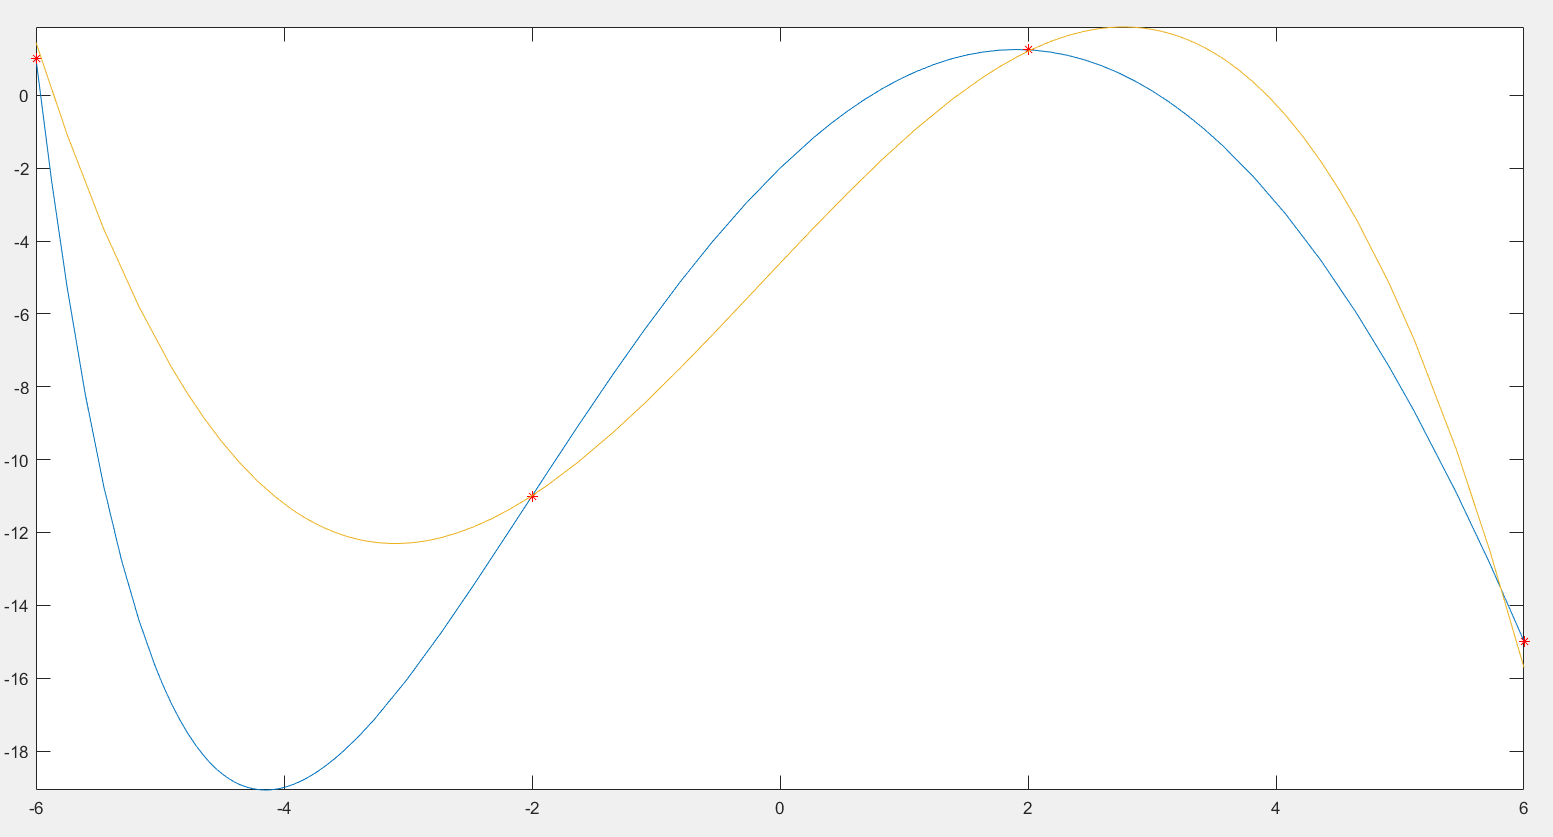
\includegraphics[scale = 0.4]{Тестовый пример}
	\end{center}
	\underline{Чебышевская сетка:}
	\begin{center}
		\begin{tabular}{|c|c|c|c|c|}
			\hline
			$x_i$ & -5.5433 & -2.2961 & 2.2961 & 5.5433 \\ \hline
			$y_i$ & -9.2681 & -12.5452 & 1.1159 & -11.5334 \\ 
			\hline
		\end{tabular}
	\end{center} 
	$$L_3(x) = 9.2681\frac{(x+2.2961)(x-2.2961)(x-5.5433)}{282.2216} - 12.5452\frac{(x+5.5433)(x-2.2961)(x-5.5433)}{116.9}-$$ $$  -1.1159\frac{(x+5.5433)(x+2.2961)(x-5.5433)}{116.9} -
	11.5334\frac{(x+5.5433)(x+2.2961)(x-2.2961)}{282.2216} = $$ $$= -0.128x^3 - 0.19x^2 + 3.6x - 4.8$$
	Ошибка в неузловой точке: $|f(0) - L_3(0)| = |-2 + 4.8| = 2.8$
	\begin{center}
		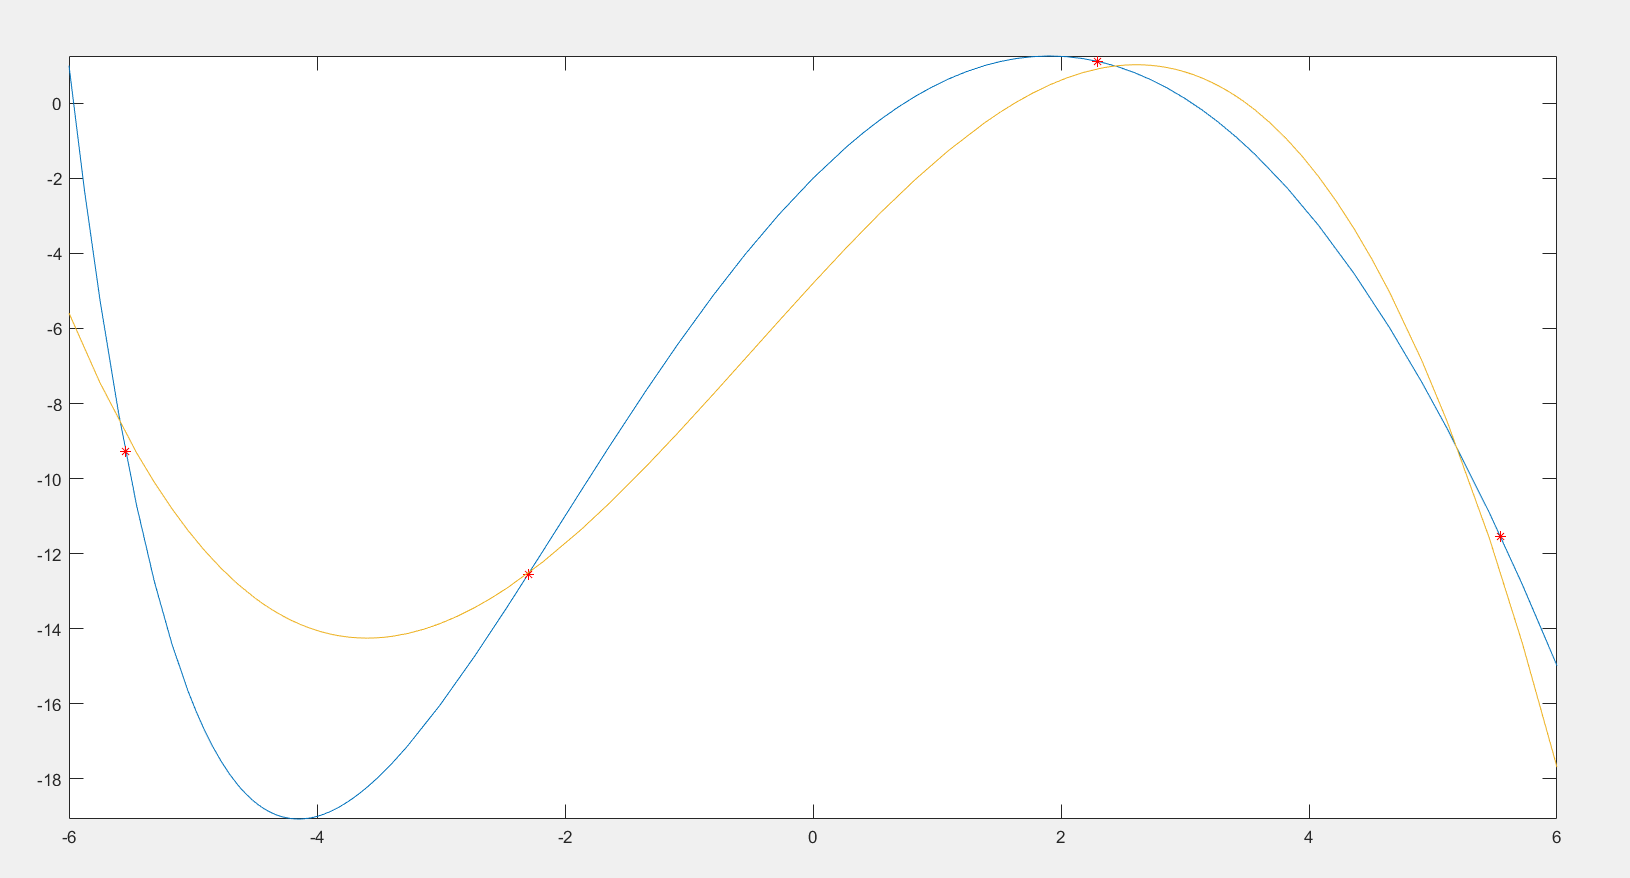
\includegraphics[scale = 0.4]{Тестовый пример Чебышев}
	\end{center}
	Мы получили $L_3(x) \approx f(x)$ для равномерной и чебышевской сетки. Интерполяция довольно не точная, но это было ожидаемо, так было задано всего 4 узла. Важно отметить, кто критерий интерполирования $\phi(x_i) = y_j$ выполняется.
	\begin{center} \textbf{Контрольные тесты}\end{center}
	\begin{enumerate}
		\item Зададим равномерную сетку и построим полином в форме Лагранжа по общей формуле для гладкой функции $f(x) = 0.5^x + 1 - (x - 2)^2$ и для функции, имеющей разрыв производной $g(x) = |f(x)|$, изменяя количество узлов(от 4 до 31).
		\item Зададим равномерную сетку и построим полином в форме Лагранжа для гладкой функции $f(x) = 0.5^x + 1 - (x - 2)^2$ по формуле для равномерной сетки, изменяя количество узлов(от 4 до 31)
	\end{enumerate}
	\begin{center} \textbf{Модульная структура программы}\end{center}
	\verb|int GetNum(ifstream *F)|\\
	\verb|vector<double> ImportData(ifstream* F, int n)|\\
	- Функции для импортирования данных\\
	\\
	\verb|double Lagrange(double x, vector<double> x_i, vector<double> y_i)|\\
	\verb|vector<double> Values(vector<double> xx, vector<double> x_i, vector<double> y_i)|\\
	- Реализация высчитывания значений полинома в форме Лагранжа по общей формуле\\
	\\
	\verb|double LagrangeUniformGrid(double x, vector<double> x_i, vector<double> y_i)|\\
	\verb|vector<double> ValuesUniformGrid(vector<double> xx, vector<double> x_i, |\\ 
	\verb|vector<double> y_i)|\\
	- Реализация высчитывания значений полинома в форме Лагранжа по формуле для равномерной сетки\\
	\\
	\verb|void OutputVector(vector<double> vec, ofstream* F)|\\
	- Функция для экспортирования данных
	\newpage
	\begin{center} \textbf{Численный анализ}\end{center}
	$\triangleright$ \underline{Общая картина:}
	\begin{center}
		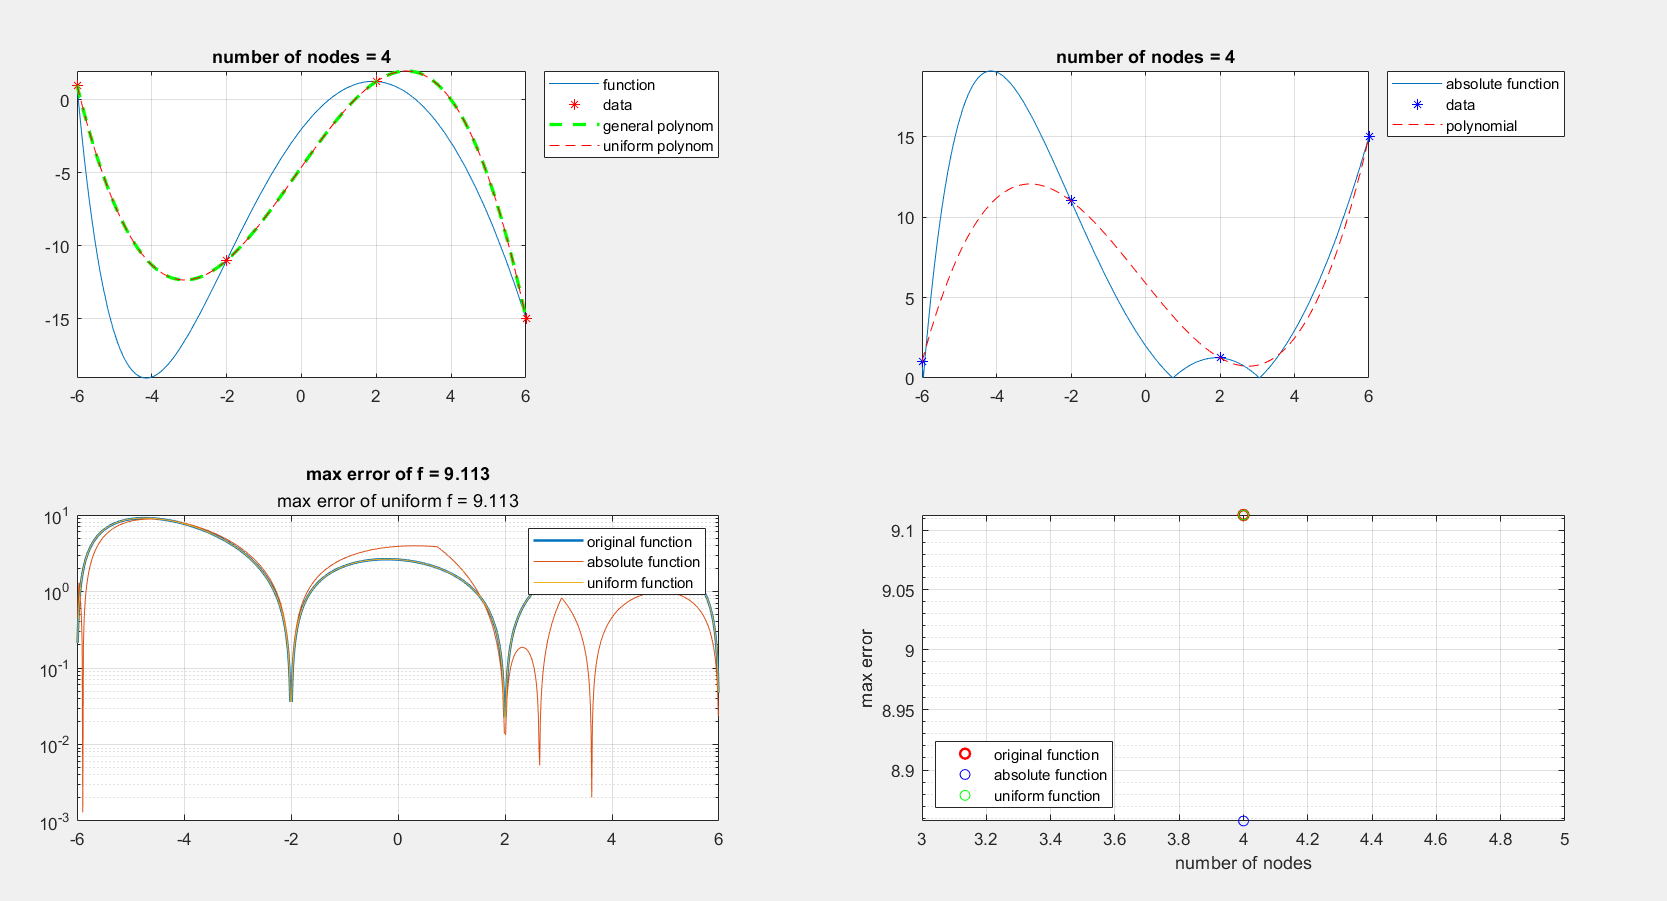
\includegraphics[scale = 0.4]{Графики1}
		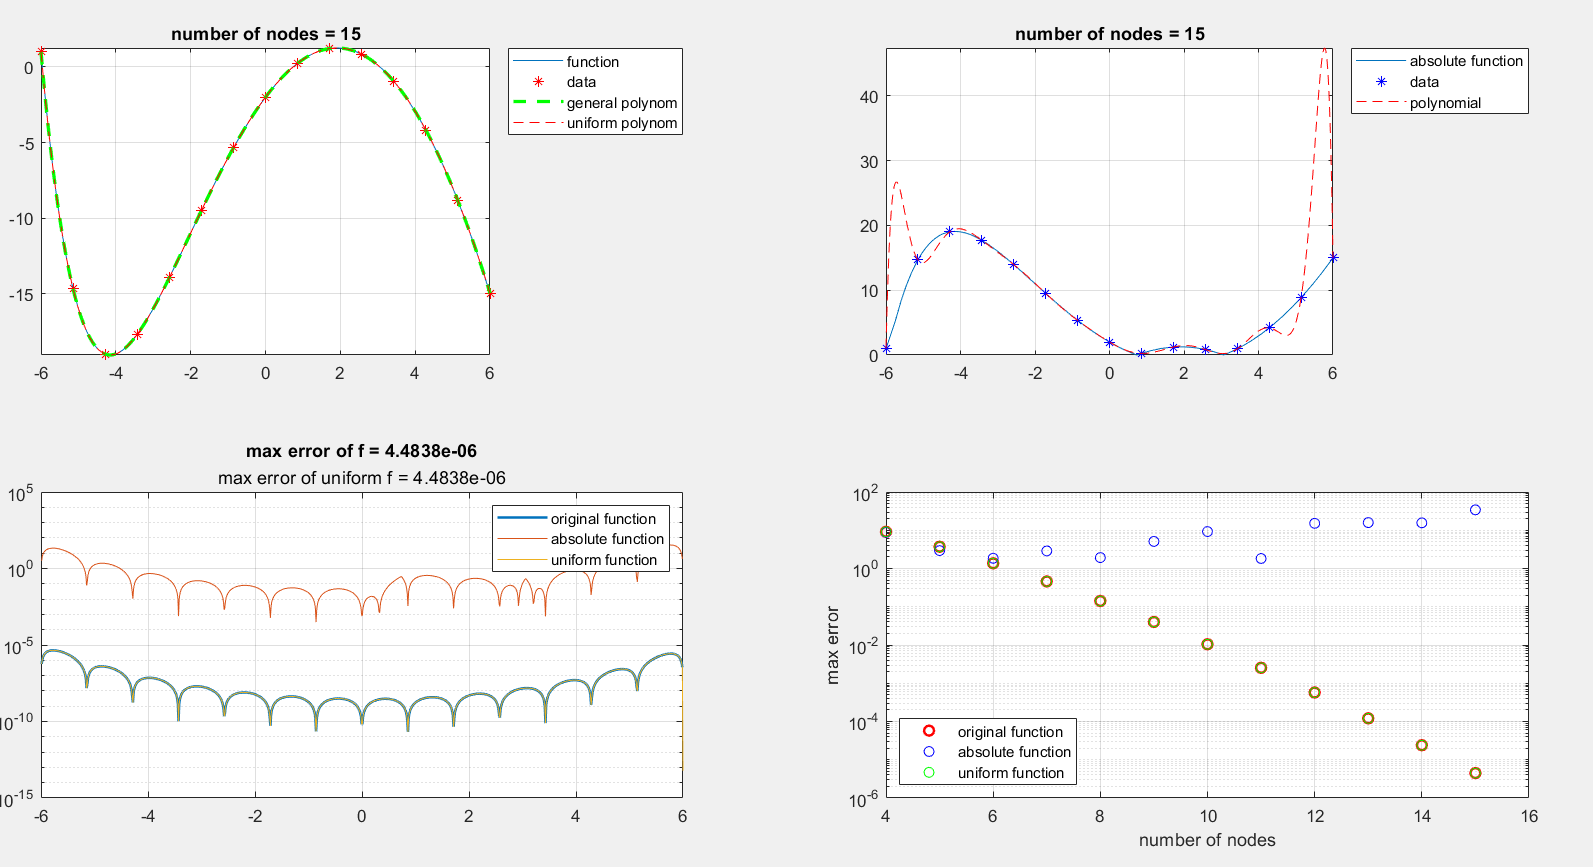
\includegraphics[scale = 0.419]{Графики2}
		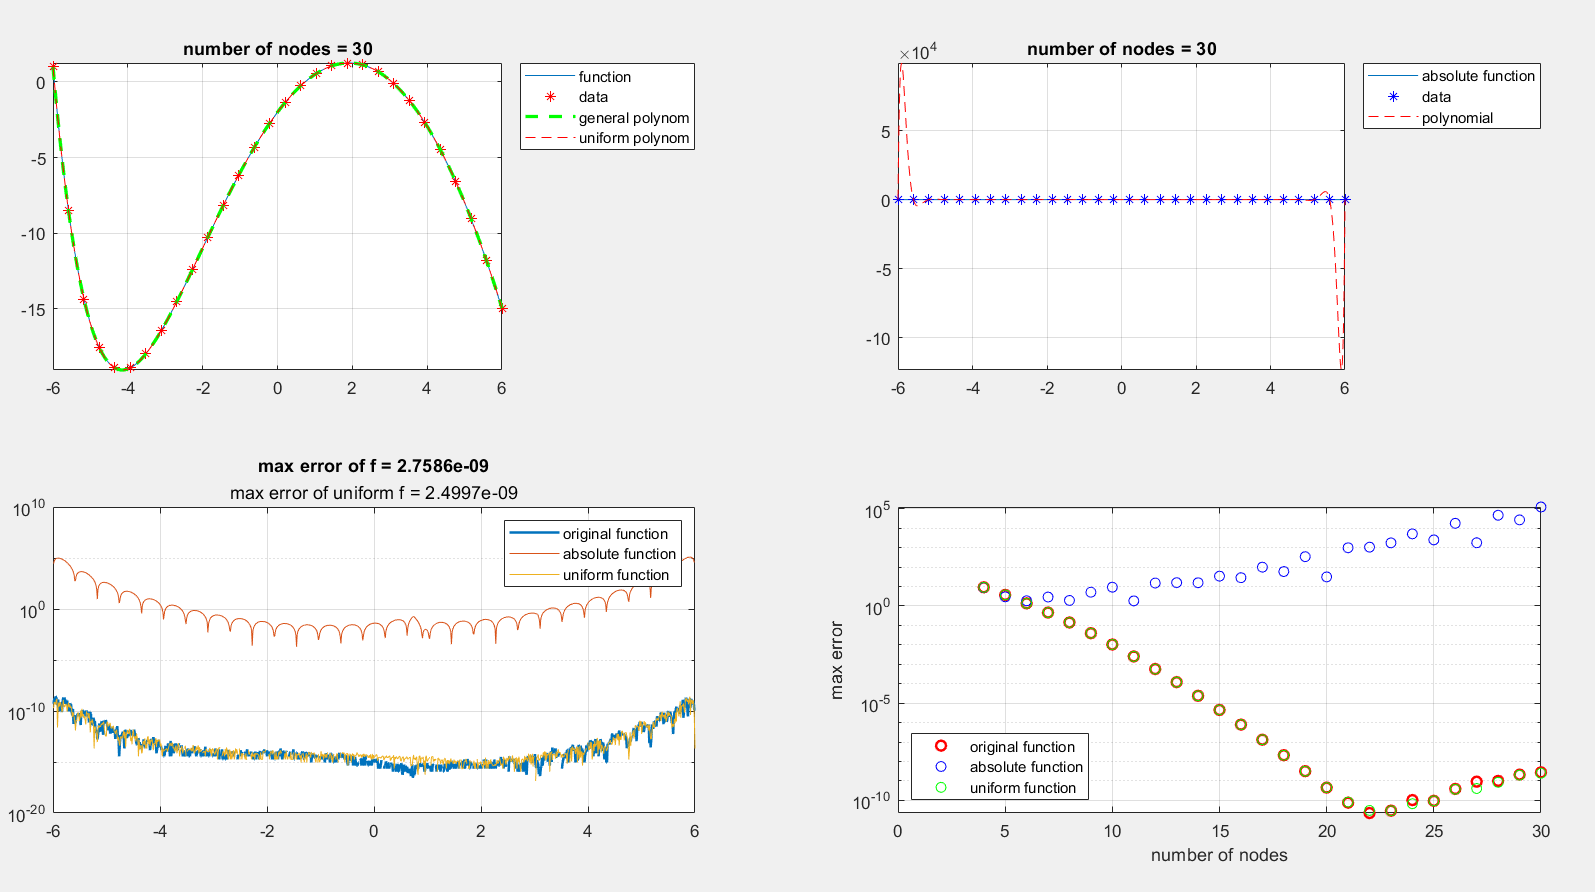
\includegraphics[scale = 0.4]{Графики3}
	\end{center}
	Из графиков видно, что разницы между построением полинома по общей формуле и по формуле для равномерной сетки нет.\\
	\\
	$\triangleright$ \underline{Приближение:}\\
	При увеличении числа узлов графики полинома все больше и больше совпадают с графиком исходной функции. Но для негладкой функции видно, что график на концах отрезка совершенно не совпадает с графиком функции.\\
	\\
	$\triangleright$ \underline{Ошибка:}\\
	При фиксированном количестве узлов ошибка в центре отрезка меньше, чем на концах. Для негладкой функции ошибка, в целом, больше ошибки для гладкой функции. Если рассматривать изменение числа узлов, то на правом нижнем графике последнего рисунка видно, что начиная с некоторого количества максимальная ошибка начинает расти.
	\begin{center} \textbf{Общие выводы}\end{center}
	В данной лабораторной работе мы научились аппроксимировать сложную функцию полиномом в форме Лагранжа. Реализация данного метода очень простая, но имеет явный недостаток - большие вычислительные затраты, например, нужно каждый раз пересчитывать все слагаемые, при изменении числа узлов, что влияет на время работы метода.
\end{document}